\documentclass[11pt]{article}
\usepackage[letterpaper,margin=0.45in]{geometry}
\usepackage{fontspec}
\usepackage{xcolor}
\usepackage{graphicx}
\usepackage{tikz}
\usepackage{tabularx}
\usepackage{enumitem}
\usepackage[hidelinks]{hyperref}
\usepackage{array}
\usepackage{ragged2e}
\usepackage[most]{tcolorbox}

\setmainfont{Helvetica Neue}
\pagestyle{empty}
\setlength{\parindent}{0pt}
\setlist[itemize]{leftmargin=1.1em,itemsep=2pt,topsep=3pt}

\definecolor{ink}{HTML}{182230}
\definecolor{muted}{HTML}{5D6B7A}
\definecolor{line}{HTML}{D9E2EC}
\definecolor{soft}{HTML}{F6F8FB}
\definecolor{dark}{HTML}{374151}

\newcommand{\slide}[1]{%
  \clearpage
  \begin{tcolorbox}[
    enhanced,
    colback=white,
    colframe=line,
    boxrule=0.6pt,
    arc=4pt,
    width=\textwidth,
    height=9.0in,
    left=14pt,
    right=14pt,
    top=14pt,
    bottom=14pt
  ]
  #1
  \end{tcolorbox}
}

\newcommand{\kicker}[1]{\textcolor{dark}{\footnotesize\bfseries\MakeUppercase{#1}}\vspace{6pt}}
\newcommand{\slidetitle}[1]{{\color{ink}\LARGE\bfseries #1}\par\vspace{12pt}}
\newcommand{\boxtitle}[1]{{\bfseries #1}\par}
\newcommand{\smallmuted}[1]{{\small\textcolor{muted}{#1}}}
\newcommand{\pill}[1]{\tikz[baseline=(x.base)]\node[fill=dark,text=white,rounded corners=3pt,inner xsep=7pt,inner ysep=4pt] (x) {\footnotesize\bfseries #1};}

\newtcolorbox{plainbox}[1][]{
  colback=white,
  colframe=line,
  boxrule=0.6pt,
  arc=4pt,
  left=9pt,
  right=9pt,
  top=8pt,
  bottom=8pt,
  #1
}

\newtcolorbox{calloutbox}{
  colback=soft,
  colframe=line,
  boxrule=0.6pt,
  arc=4pt,
  left=10pt,
  right=10pt,
  top=8pt,
  bottom=8pt
}

\begin{document}

\slide{
  \begin{center}
    {\Huge\bfseries Dreamforce}\par
    \vspace{6pt}
    {\large\textcolor{muted}{September 15--17, 2026}}\par
    \vspace{22pt}
    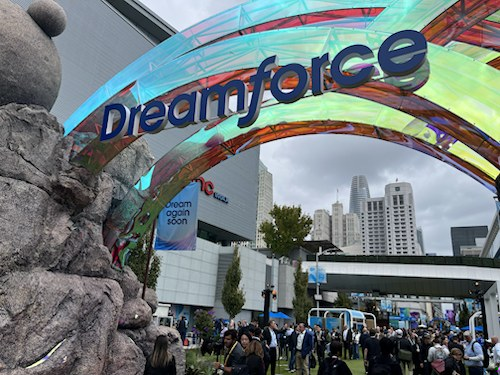
\includegraphics[width=0.88\textwidth,height=6.35in,keepaspectratio]{assets/dreamforce_cover/IMG_1575.jpg}
  \end{center}
}

\slide{
  \kicker{Salesforce Product Stack}\par
  \smallmuted{AI Force and Agentforce sit above Customer 360; Slack and Tableau remain adjacent collaboration and analytics tools.}
  \vspace{12pt}
  \begin{center}
  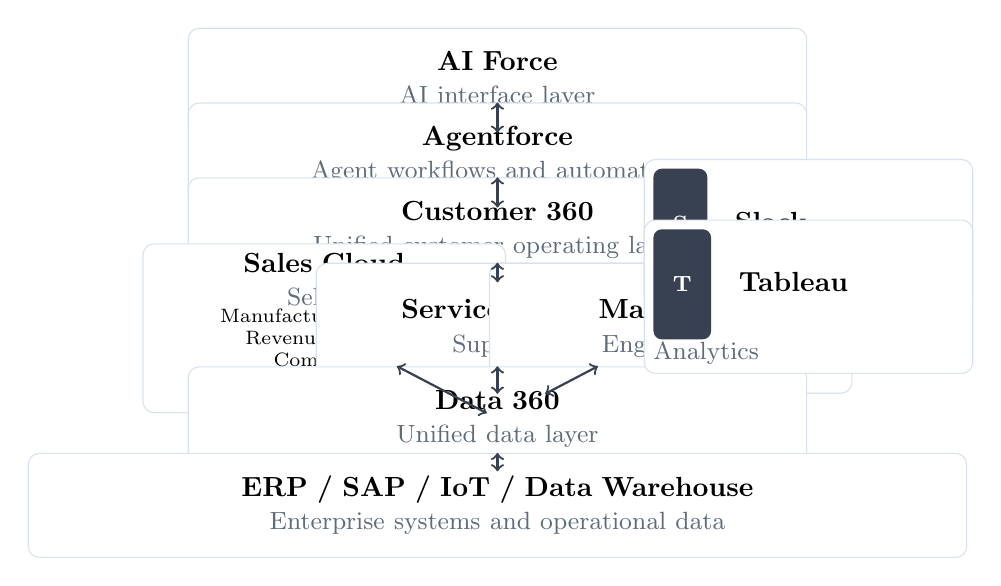
\begin{tikzpicture}[
    box/.style={draw=line, fill=white, rounded corners=4pt, minimum height=0.52in, align=center, text width=3.0in},
    smallbox/.style={draw=line, fill=white, rounded corners=4pt, minimum height=0.65in, align=center, text width=1.72in},
    tool/.style={draw=line, fill=white, rounded corners=4pt, minimum height=0.55in, align=left, text width=1.55in},
    arrow/.style={-latex, thick, draw=dark}
  ]
    \node[box] (ai) at (0,5.4) {\boxtitle{AI Force}\smallmuted{AI interface layer}};
    \node[box] (agent) at (0,4.45) {\boxtitle{Agentforce}\smallmuted{Agent workflows and automation}};
    \node[box] (cust) at (0,3.5) {\boxtitle{Customer 360}\smallmuted{Unified customer operating layer}};
    \node[smallbox] (sales) at (-2.2,2.25) {\boxtitle{Sales Cloud}\smallmuted{Selling}\\[-2pt]\scriptsize Manufacturing Cloud\\Revenue / CPQ\\Commerce\\Experience Cloud};
    \node[smallbox] (service) at (0,2.25) {\boxtitle{Service Cloud}\smallmuted{Support}};
    \node[smallbox] (mkt) at (2.2,2.25) {\boxtitle{Marketing}\smallmuted{Engagement}};
    \node[box] (data) at (0,1.1) {\boxtitle{Data 360}\smallmuted{Unified data layer}};
    \node[box, text width=4.6in] (erp) at (0,0) {\boxtitle{ERP / SAP / IoT / Data Warehouse}\smallmuted{Enterprise systems and operational data}};
    \draw[arrow,<->] (ai) -- (agent);
    \draw[arrow,<->] (agent) -- (cust);
    \draw[arrow,<->] (cust) -- (service);
    \draw[arrow,<->] (sales) -- (data);
    \draw[arrow,<->] (service) -- (data);
    \draw[arrow,<->] (mkt) -- (data);
    \draw[arrow,<->] (data) -- (erp);
    \node[tool] at (3.95,3.45) {\pill{S}\quad \boxtitle{Slack}\smallmuted{Collaboration}};
    \node[tool] at (3.95,2.65) {\pill{T}\quad \boxtitle{Tableau}\smallmuted{Analytics}};
  \end{tikzpicture}
  \end{center}
  \vfill
  \begin{tabularx}{\textwidth}{XXXX}
    \textbf{AI Force}\newline\smallmuted{Interface layer} &
    \textbf{Agentforce}\newline\smallmuted{Agentic workflows} &
    \textbf{Customer 360}\newline\smallmuted{Business apps} &
    \textbf{Data 360}\newline\smallmuted{Unified data}
  \end{tabularx}
}

\slide{
  \kicker{Enterprise Context}\par
  \slidetitle{Two CRM Patterns to Consider}
  \begin{tabularx}{\textwidth}{XX}
    \begin{plainbox}
      \centering
      \boxtitle{Clean Core CRM}\vspace{8pt}
      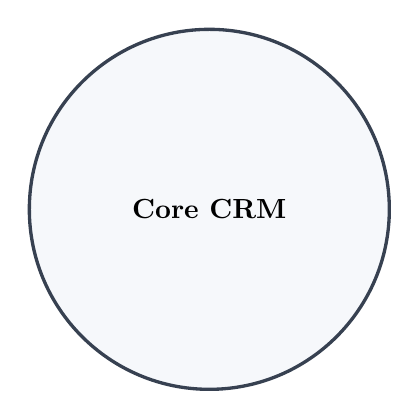
\begin{tikzpicture}
        \draw[dark, line width=1.2pt, fill=soft] (0,0) circle (0.9in);
        \node[align=center] at (0,0) {\bfseries Core CRM};
      \end{tikzpicture}
      \vspace{8pt}
      \smallmuted{Sales function enabled by a cleaner, more complete CRM operating model.}
    \end{plainbox}
    &
    \begin{plainbox}
      \centering
      \boxtitle{Minimal CRM + Agentic Layer}\vspace{8pt}
      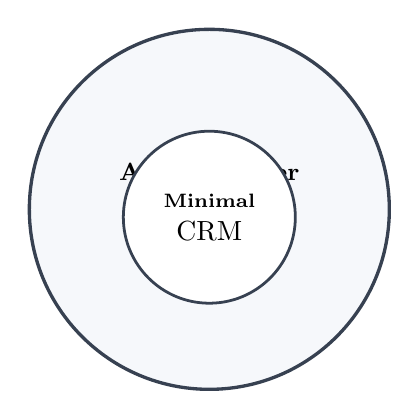
\begin{tikzpicture}
        \draw[dark, line width=1.2pt, fill=soft] (0,0) circle (0.9in);
        \node[align=center] at (0,0.45) {\small\bfseries Agentic Layer};
        \draw[dark, line width=1.0pt, fill=white] (0,-0.1) circle (0.43in);
        \node[align=center] at (0,-0.1) {\scriptsize\bfseries Minimal\\CRM};
      \end{tikzpicture}
      \vspace{8pt}
      \smallmuted{Lightweight CRM foundation integrated with agents to enable business functions.}
    \end{plainbox}
  \end{tabularx}
  \vspace{14pt}
  \begin{center}
  \begin{plainbox}[width=5.3in]
    \kicker{Decision Criteria}\par
    \begin{center}
    \begin{tikzpicture}[x=1in,y=1in]
      \draw[dark, thick] (0,0) -- (4.2,0);
      \draw[dark, thick] (0,0) -- (0,2.15);
      \draw[line, thick] (2.1,0) -- (2.1,2.15);
      \draw[line, thick] (0,1.075) -- (4.2,1.075);
      \node[below] at (0.25,0) {\scriptsize Low};
      \node[below] at (3.95,0) {\scriptsize High};
      \node[left] at (0,0.22) {\scriptsize Low};
      \node[left] at (0,1.95) {\scriptsize High};
      \node[below=0.28in] at (2.1,0) {\small\bfseries Maintainability};
      \node[rotate=90] at (-0.52,1.075) {\small\bfseries Maturity};
      \fill[dark] (3.55,1.78) circle (4pt);
      \node[draw=line, fill=white, rounded corners=3pt, anchor=west] at (3.65,1.78) {\scriptsize\bfseries Ideal solution};
    \end{tikzpicture}
    \end{center}
    \small \textbf{Maturity:} evidence of successful implementation. \hfill
    \textbf{Maintainability:} easier to operate, govern, and evolve.
  \end{plainbox}
  \end{center}
}

\slide{
  \kicker{Key Takeaway 1}\par
  \slidetitle{Headless Agent Experiences Are a Major Theme}
  \begin{tabularx}{\textwidth}{XX}
    \begin{plainbox}
      \boxtitle{Headless Experience}
      \begin{itemize}
        \item Experience is not tied to one Salesforce screen.
        \item Agents can surface in Slack, web, mobile, Claude, or custom apps.
        \item The interface changes; Salesforce remains the workflow/data engine.
      \end{itemize}
    \end{plainbox}
    &
    \begin{plainbox}
      \boxtitle{MCP + Agent Workflows}
      \begin{itemize}
        \item MCP was shown as a way for agents to connect to tools and systems.
        \item Agent workflows were prominent across demos and technical sessions.
        \item Salesforce is promoting agent building on its own platform stack.
      \end{itemize}
    \end{plainbox}
  \end{tabularx}
  \vspace{18pt}
  \begin{center}
    \begin{tabular}{ccc}
      \begin{plainbox}[width=1.9in]\boxtitle{Any Interface}\smallmuted{Slack, web, Claude, apps}\end{plainbox}
      & \(\rightarrow\) &
      \begin{plainbox}[width=1.9in]\boxtitle{Agentforce}\smallmuted{Agent reasoning + workflow}\end{plainbox}
      \\[10pt]
      && \(\rightarrow\) \quad
      \begin{plainbox}[width=1.9in]\boxtitle{MCP / Tools}\smallmuted{Systems, actions, data}\end{plainbox}
    \end{tabular}
  \end{center}
  \vfill
  \begin{calloutbox}
    \textbf{Short definition:} A headless experience separates the user interface from the backend workflow. Users may interact through Slack, Claude, a website, or another app while Salesforce powers the data, permissions, workflow, and agent actions behind the scenes.
  \end{calloutbox}
}

\slide{
  \kicker{Key Takeaway 2}\par
  \slidetitle{Slack Is the Preferred Agentic Work Surface}
  \begin{tabularx}{\textwidth}{XX}
    \begin{plainbox}
      \boxtitle{Strong Salesforce + Slack Native Integration}
      \begin{itemize}
        \item Slack positioned as the collaboration layer for agents.
        \item Agentic development is heavily promoted through Slack workflows.
        \item Best fit for alerts, approvals, summaries, and team handoffs.
      \end{itemize}
    \end{plainbox}
    &
    \begin{plainbox}
      \boxtitle{Microsoft Teams Integration Appears Less Mature}
      \begin{itemize}
        \item No visible Microsoft presence in the enterprise section observed.
        \item Teams was not highlighted as the primary agentic interface.
        \item Integration may require more validation before enterprise rollout.
      \end{itemize}
    \end{plainbox}
  \end{tabularx}
  \vspace{18pt}
  \begin{center}
    \begin{tabular}{ccccc}
      \begin{plainbox}[width=1.8in]\boxtitle{Salesforce Data}\smallmuted{CRM + customer context}\end{plainbox}
      & \(\rightarrow\) &
      \begin{plainbox}[width=1.7in]\boxtitle{Agentforce}\smallmuted{Reason, summarize, act}\end{plainbox}
      & \(\rightarrow\) &
      \begin{plainbox}[width=1.55in]\boxtitle{Slack}\smallmuted{Team execution surface}\end{plainbox}
    \end{tabular}
  \end{center}
  \vfill
  \begin{calloutbox}
    \textbf{Implication:} For Salesforce-led agent pilots, Slack should be treated as the default collaboration interface. Teams integration should be assessed separately for maturity, roadmap fit, and operational friction.
  \end{calloutbox}
}

\slide{
  \kicker{Key Takeaway 3}\par
  \slidetitle{AIforce Branding Is Most Visible Through Claude}
  \begin{tabularx}{\textwidth}{XX}
    \begin{plainbox}
      \boxtitle{Claude / Claudeforce}
      \begin{itemize}
        \item Official Salesforce launch centers Claude via Claudeforce.
        \item Salesforce in Claude brings CRM context and sales skills into Claude.
        \item Claude docs confirm support in Claude Cowork.
      \end{itemize}
    \end{plainbox}
    &
    \begin{plainbox}
      \boxtitle{ChatGPT / Gemini}
      \begin{itemize}
        \item AIforce is described as open to any AI interface.
        \item Salesforce references OpenAI and Google in the ecosystem.
        \item Event messaging made Claude more explicit than ChatGPT or Gemini.
      \end{itemize}
    \end{plainbox}
  \end{tabularx}
  \vspace{10pt}
  \begin{center}
    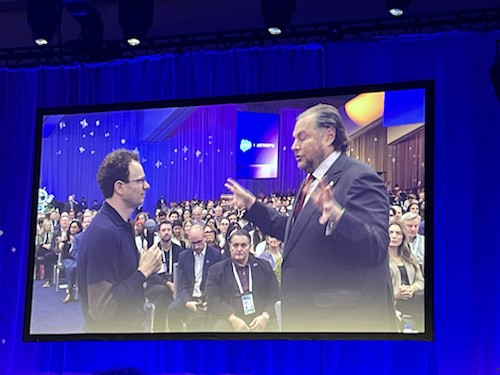
\includegraphics[width=0.82\textwidth,height=2.65in,keepaspectratio]{assets/dreamforce_cover/IMG_1528.jpg}
  \end{center}
  \vfill
  \begin{calloutbox}
    \textbf{Verified:} Claude is the clearest branded integration path: Claudeforce and Salesforce in Claude. ChatGPT and Gemini are visible in AIforce's broader open-interface ecosystem, but were less obvious in the primary launch narrative.
  \end{calloutbox}
}

\slide{
  \kicker{Key Takeaway 4}\par
  \slidetitle{Zero-Copy Integration with Snowflake and Databricks}
  \begin{tabularx}{\textwidth}{XX}
    \begin{plainbox}
      \boxtitle{Snowflake}
      \begin{itemize}
        \item Salesforce Data 360 supports zero-copy sharing with Snowflake.
        \item Data can be queried without ETL pipelines or duplication.
        \item Useful for analytics, ML, and AI apps using Salesforce context.
      \end{itemize}
    \end{plainbox}
    &
    \begin{plainbox}
      \boxtitle{Databricks}
      \begin{itemize}
        \item Data 360 supports zero-copy access patterns for Databricks.
        \item Data 360 zero-copy connectors are alternatives to ingestion.
        \item Good fit for lakehouse analytics and AI/ML workloads.
      \end{itemize}
    \end{plainbox}
  \end{tabularx}
  \vspace{10pt}
  \begin{tabularx}{\textwidth}{XXX}
    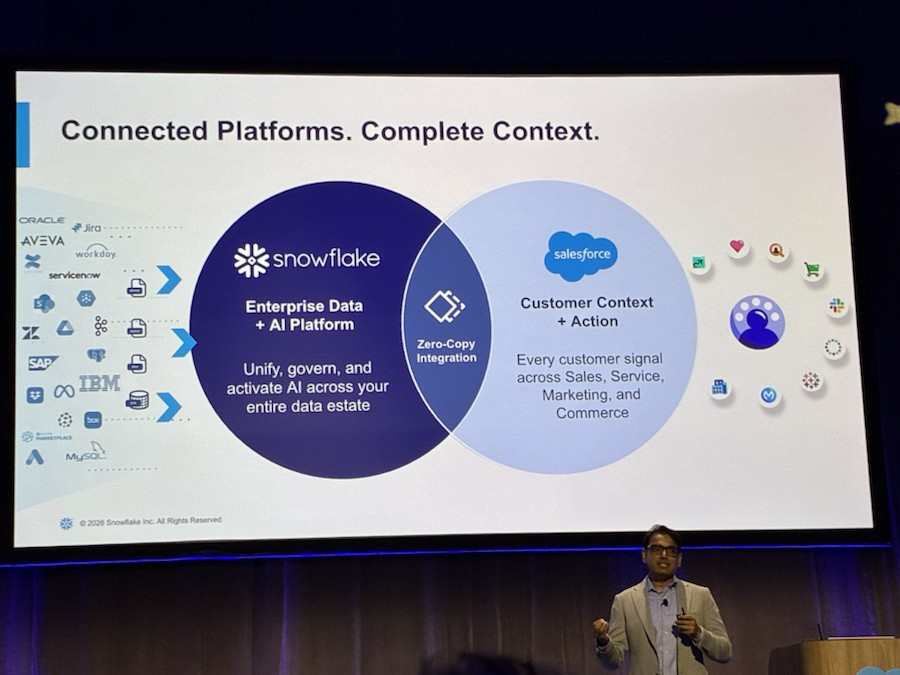
\includegraphics[width=\linewidth]{assets/dreamforce_cover/IMG_0009.jpg} &
    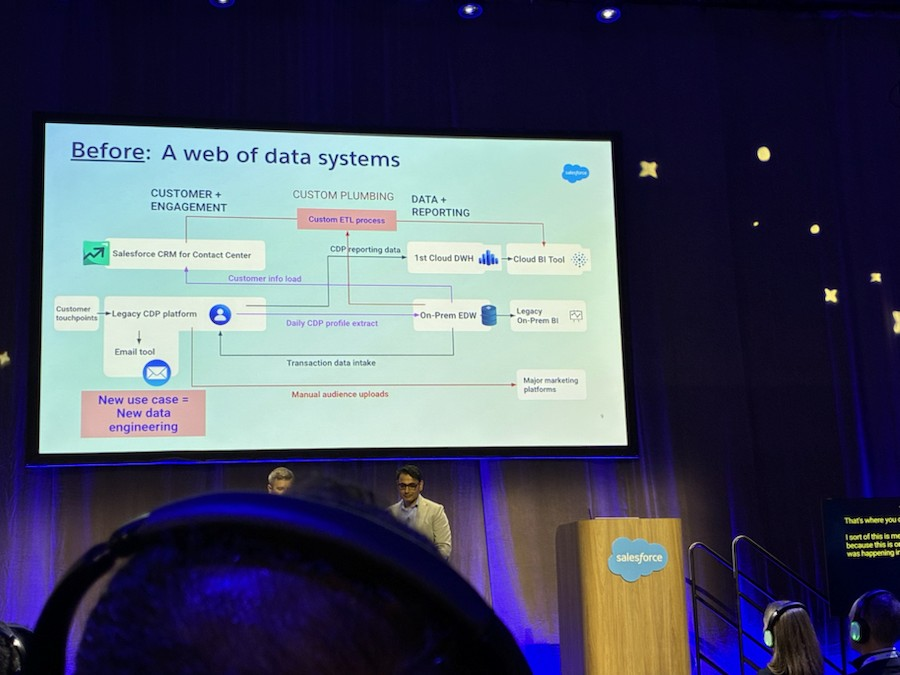
\includegraphics[width=\linewidth]{assets/dreamforce_cover/IMG_0013.jpg} &
    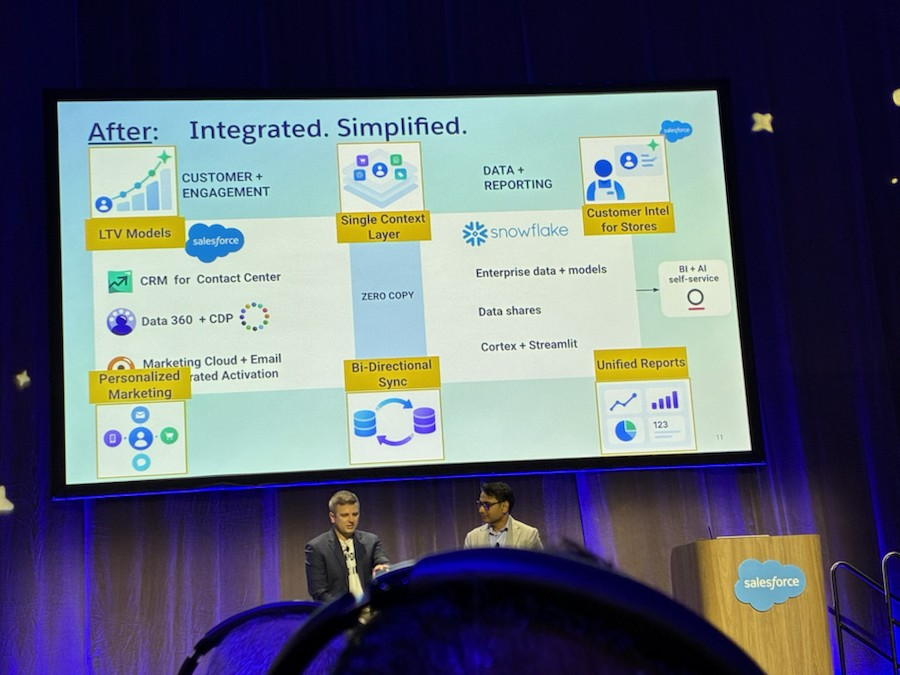
\includegraphics[width=\linewidth]{assets/dreamforce_cover/IMG_0015.jpg}
  \end{tabularx}
  \vspace{12pt}
  \begin{center}
    \begin{tabular}{ccccc}
      \begin{plainbox}[width=1.55in]\boxtitle{Snowflake}\smallmuted{Warehouse}\end{plainbox}
      & \(\leftrightarrow\) &
      \begin{plainbox}[width=1.55in]\boxtitle{Data 360}\smallmuted{Federation + sharing}\end{plainbox}
      & \(\leftrightarrow\) &
      \begin{plainbox}[width=1.55in]\boxtitle{Databricks}\smallmuted{Lakehouse}\end{plainbox}
    \end{tabular}
  \end{center}
  \vfill
  \begin{calloutbox}
    \textbf{Verified:} Salesforce, Snowflake, and Databricks documentation support zero-copy integration patterns. Practical takeaway: less ETL, less duplication, fresher data; setup, permissions, and governance still need architecture review.
  \end{calloutbox}
}

\slide{
  \kicker{Key Takeaway 5}\par
  \slidetitle{Siemens Appeared as a Core Demo Partner}
  \begin{tabularx}{\textwidth}{XX}
    \begin{plainbox}
      \boxtitle{Supplier Onboarding on SAP}
      \begin{itemize}
        \item Demo showed supplier onboarding tied to SAP.
        \item Signals Salesforce interest in enterprise process integration.
        \item Relevant to ERP-adjacent workflows, not only CRM use cases.
      \end{itemize}
    \end{plainbox}
    &
    \begin{plainbox}
      \boxtitle{Piper Sales Website Agent}
      \begin{itemize}
        \item Demo included a sales website application built with a Salesforce agent.
        \item Piper demonstrated guided selling / buyer interaction potential.
        \item Shows agent capabilities moving into digital sales experiences.
      \end{itemize}
    \end{plainbox}
  \end{tabularx}
  \vspace{10pt}
  \begin{tabularx}{\textwidth}{XX}
    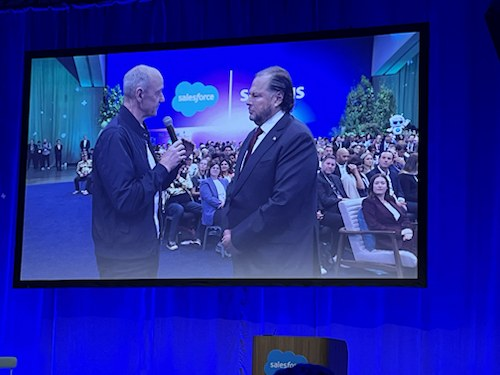
\includegraphics[width=\linewidth,height=1.85in,keepaspectratio]{assets/dreamforce_cover/IMG_1531.jpg} &
    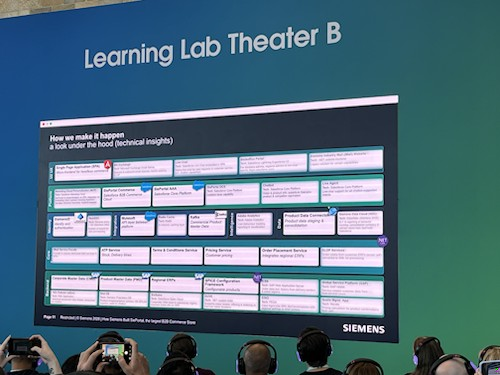
\includegraphics[width=\linewidth,height=1.85in,keepaspectratio]{assets/dreamforce_cover/IMG_1549.jpg}
  \end{tabularx}
  \vspace{12pt}
  \begin{center}
    \begin{tabular}{ccccc}
      \begin{plainbox}[width=1.45in]\boxtitle{Siemens}\smallmuted{Demo partner signal}\end{plainbox}
      & \(\rightarrow\) &
      \begin{plainbox}[width=1.45in]\boxtitle{SAP}\smallmuted{Supplier onboarding}\end{plainbox}
      & \(\rightarrow\) &
      \begin{plainbox}[width=1.45in]\boxtitle{Piper}\smallmuted{Sales website agent}\end{plainbox}
    \end{tabular}
  \end{center}
  \vfill
  \begin{calloutbox}
    \textbf{Implication:} Salesforce is showcasing agentic capabilities through realistic enterprise scenarios: SAP process integration and customer-facing sales applications. Siemens may be a useful reference pattern for industrial and complex B2B workflows.
  \end{calloutbox}
}

\slide{
  \kicker{Top Recommendations}\par
  \slidetitle{Prioritize ROI, Fit, Partners, and Data}
  \begin{tabularx}{\textwidth}{XX}
    \begin{plainbox}
      \boxtitle{1. Adopt Selectively, Then Use Consistently}
      \smallmuted{Even 10--15\% of the demonstrated features can deliver high ROI if implemented well and used consistently.}
    \end{plainbox}
    &
    \begin{plainbox}
      \boxtitle{2. Let Sales Use Cases Drive Stack Choices}
      \smallmuted{Many features are superfluous for our industry and growth stage. Choose products based on concrete Sales workflows.}
    \end{plainbox}
    \\[10pt]
    \begin{plainbox}
      \boxtitle{3. Use Enterprise Partners for Complex Logic}
      \smallmuted{Agentic use cases with complex business rules will likely require experienced implementation partners.}
    \end{plainbox}
    &
    \begin{plainbox}
      \boxtitle{4. Prioritize the Integrated Data Layer}
      \smallmuted{Highest value: extract relevant Salesforce account data in Snowflake, analyze on Databricks, and use zero-copy access for an agentic application.}
    \end{plainbox}
  \end{tabularx}
  \vfill
  \begin{calloutbox}
    \textbf{Potential partner:} Vigience, for Salesforce/SAP integration evaluation. Website: \href{https://www.vigience.com/}{vigience.com}.
  \end{calloutbox}
}

\end{document}
